\documentclass[conference]{IEEEtran}
\IEEEoverridecommandlockouts
% The preceding line is only needed to identify funding in the first footnote. 
% If that is unneeded, please comment it out.
\usepackage{cite}
\usepackage{amsmath,amssymb,amsfonts}
\usepackage{algorithmic}
\usepackage{graphicx}
\usepackage{textcomp}
\usepackage{xcolor}
\usepackage[linesnumbered,ruled,vlined]{algorithm2e}
\usepackage{hyperref}
\usepackage{booktabs}
\usepackage{makecell}
\usepackage{multirow}

\DeclareRobustCommand*{\IEEEauthorrefmark}[1]{%
    \raisebox{0pt}[0pt][0pt]{\textsuperscript{\footnotesize\ensuremath{#1}}}}

\def\BibTeX{{\rm B\kern-.05em{\sc i\kern-.025em b}\kern-.08em
    T\kern-.1667em\lower.7ex\hbox{E}\kern-.125emX}}
\begin{document}

\title{DyCoT‑RE: Chain-of-Thought-Enhanced LLM Reward Engineering with Dual-Dynamic Optimization for Reinforcement Learning}


\author{
\IEEEauthorblockN{1\textsuperscript{st} Xinning Zhu}
\IEEEauthorblockA{\textit{Sino-European School of Technology} \\
\textit{Shanghai University}\\
Shanghai, China \\
zhuxinning@shu.edu.cn}
~\\
\and
\IEEEauthorblockN{2\textsuperscript{nd} Jinxin Du}
\IEEEauthorblockA{\textit{Sino-European School of Technology} \\
\textit{Shanghai University}\\
Shanghai, China \\
jinxin\_du@shu.edu.cn}
~\\
\and
\IEEEauthorblockN{3\textsuperscript{th} Lunde Chen*}
\IEEEauthorblockA{\textit{Sino-European School of Technology} \\
\textit{Shanghai University}\\
Shanghai, China \\
lundechen@shu.edu.cn}
*Corresponding author
}

\maketitle

\begin{abstract}
Designing effective reward functions remains a challenge in applying reinforcement learning to real-world tasks.
This paper proposes DyCoT-RE, a reward engineering framework that integrates Chain-of-Thought (CoT) reasoning with a dual-dynamic 
optimization strategy to automate and enhance reward function design.
The framework uses structured CoT reasoning throughout training to generate and refine interpretable reward code in each iteration.
It further incorporates a dual-dynamic optimization mechanism: a temperature adjustment strategy that modulates the sampling temperature 
based on policy entropy trends,
and a model switching strategy that allocates language models with different capabilities to produce distinct reward components.
Evaluations on CartPole, BipedalWalker, Ant, and a custom SpaceMining environment show DyCoT‑RE achieves higher average rewards and faster 
convergence compared to human-designed baselines and non‑CoT approaches as well as single-optimization approaches.


\end{abstract}

\begin{IEEEkeywords}
Reinforcement learning, reward engineering, large language models, chain-of-thought reasoning, dynamic temperature adjustment, model selection
\end{IEEEkeywords}

\section{Introduction}

Reinforcement learning (RL) has achieved impressive results across diverse domains 
However, as Sutton et al. \cite{sutton1998reinforcement} emphasize, the reward signal is the primary means of specifying task objectives in RL, making its design critical to achieving desired behaviors.
In practice, translating intended behaviors into precise, effective reward functions remains highly challenging, particularly for tasks involving long-term dependencies 
\cite{amodei2016concrete}.
Skalse et al. \cite{skalse2022misspecification} demonstrate that agents often exploit imperfections in reward formulations to maximize proxy objectives in unintended ways, leading to behaviors that optimize the designed reward but undermine true task performance.
These challenges highlight that despite RL’s theoretical versatility, its practical deployment is often constrained by the complexity, subtlety, and domain expertise required for robust reward engineering \cite{ibarz2018reward}.

While carefully designed rewards can accelerate agent learning and improve task performance,
manual reward engineering typically relies on trial-and-error tuning,
which is labor-intensive and often yields suboptimal generalization to new environments or objectives \cite{hadfield2017inverse}..
As RL applications grow in complexity, there is a pressing need for methods that can automate
reward design while maintaining interpretability and flexibility.

Recent advances in large language models (LLMs) have demonstrated strong reasoning and generalization capabilities \cite{brown2020language, ouyang2022training}.
In particular, Chain-of-Thought (CoT) reasoning enables LLMs to decompose tasks into structured intermediate steps,
enhancing clarity and alignment with desired objectives \cite{wei2022chain}.
This structured reasoning process can support reward engineering by converting task descriptions
into executable reward functions in a systematic and transparent manner.

However, existing CoT-based reward generation approaches typically use static sampling parameters and fixed model configurations,
which may limit their adaptability during training.
Motivated by recent progress in dynamic temperature adjustment and model selection strategies\cite{zhu2024hot, fedus2022switch},
we explore whether integrating adaptive optimization mechanisms into CoT-based reward generation
can improve reward quality, training stability, and sampling efficiency.
Dynamic temperature modulation can adjust exploration levels throughout training \cite{zhang2024edt},
while model selection strategies can allocate LLMs with specialized capabilities to different reward generation tasks \cite{du2022glam}.

In this work, we propose DyCoT-RE, a reward engineering framework that integrates structured CoT reasoning
with dual-dynamic optimization.
Specifically, DyCoT-RE leverages CoT reasoning to decompose natural language task descriptions into structured reward components,
then employs iterative refinement to enhance alignment with learning objectives.
The dual-dynamic optimization strategy integrates entropy-guided temperature adjustment to balance exploration and exploitation,
alongside a dynamic model selection module that routes sub-tasks to specialized LLMs based on performance feedback.
By tightly coupling these components within a closed-loop evolutionary search process, 
DyCoT-RE systematically improves reward function quality and training efficiency,
ultimately enabling scalable, interpretable, and automated reward engineering for complex RL environments.


We evaluate DyCoT-RE on four standard RL environments—CartPole, BipedalWalker, and Ant—
as well as a custom SpaceMining environment.
Results show that DyCoT-RE achieves improved average rewards and faster convergence compared to baselines and non-CoT methods.

The remainder of this paper is organized as follows.
Section II reviews related work in reward engineering, LLM-based reward generation, and adaptive optimization.
Section III describes the proposed methodology, including the CoT reward framework, temperature adjustment, and model selection.
Section IV details the experimental setup, and Section V presents results and analysis.
Section VI discusses limitations and future work, with Section VII concluding the paper.

\section{Related Work}

\subsection{Reward Engineering Paradigms}

In RL, the design of effective reward functions directly shapes agent behavior and learning outcomes. 
Traditional approaches primarily rely on handcrafted reward functions informed by domain expertise. 
While intuitive, such manual design often struggles to capture complex, dynamic task objectives and is prone to 
suboptimal or biased formulations, hindering agent performance in real-world scenarios.

To address these limitations, reward shaping was introduced as a formal enhancement strategy. 
Ng et al. \cite{ng1999policy} demonstrated that potential-based reward shaping preserves optimal policies 
while enabling accelerated convergence, laying the theoretical foundation for numerous practical implementations. 
Intrinsic motivation frameworks further advanced this field by encouraging exploration through curiosity-driven signals. 
Singh et al. \cite{singh2010intrinsically} proposed intrinsic rewards to incentivize novel state visits, 
later extended by Burda et al. \cite{burda2018exploration}, who empirically validated large-scale curiosity-driven exploration 
benefits across diverse environments.

Despite these developments, manually designing rewards for complex or evolving tasks remains inefficient and costly. 
LLMs offer a promising alternative by leveraging their natural language understanding to automate reward generation 
and optimization. Unlike traditional RL pipelines that require explicit, task-specific reward formulations, 
LLMs can interpret high-level task descriptions, extract key objectives, and translate them into executable reward functions. 
This capability facilitates more intuitive alignment with human intentions, reduces engineering overhead, and enhances agent 
adaptability.

Recent frameworks exemplify this trend. EUREKA \cite{ma2023eureka}, Text2Reward \cite{xie2023text2reward}, 
CARD \cite{sun2024large}, and PCGRLLM \cite{baek2024pcgrllm} harness LLMs to automatically generate, verify, 
and refine reward code from natural language instructions. Notably, PCGRLLM extends this capability to procedural content 
generation tasks, demonstrating that LLM-driven reward design can generalize beyond standard control problems to complex 
creative domains such as game level generation.


Beyond static code generation, feedback-driven optimization approaches have emerged. ReMiss \cite{xie2024jailbreaking} 
utilizes adversarial prompt generation to identify and mitigate reward misspecification vulnerabilities, 
enhancing LLM safety and reliability. Self-Play Preference Optimization (SPPO) \cite{wu2024self} employs self-play to 
uncover Nash-equilibrium strategies that capture complex, non-transitive human preferences, advancing preference learning's 
applicability in RL. 
Additionally, PRMBench \cite{song2025prmbench} provides a process-level benchmark to evaluate intermediate reward model 
outputs along dimensions such as conciseness, rationality, and sensitivity, revealing weaknesses in current models and 
guiding future improvements.

Overall, LLM-based reward engineering represents a paradigm shift. 
By integrating natural language reasoning and dynamic feedback optimization, 
these methods offer scalable, adaptable, and human-aligned reward generation pipelines. 
As tasks grow in complexity and diversity, leveraging LLMs to bridge the gap between human 
intent and machine learning objectives will be critical for the next generation of intelligent systems. 
Continued research is thus needed to maximize the synergy between LLM capabilities and RL frameworks to 
address emerging real-world challenges.

\subsection{Chain-of-Thought Reasoning Methods}

CoT reasoning has emerged as a powerful paradigm to enhance the reasoning capabilities of LLMs. 
By generating intermediate reasoning steps, CoT allows models to decompose complex problems into interpretable sub-problems, 
leading to significant performance gains in tasks requiring multi-step logical inference.

Early studies showed that even simple prompting strategies, such as adding ``Let's think step by step,'' 
can elicit strong zero-shot reasoning abilities. Kojima et al. \cite{kojima2022large} demonstrated such prompts 
significantly improve performance in arithmetic and commonsense tasks. 
Building upon this, few-shot CoT \cite{wei2022chain} introduced demonstrations of stepwise solutions to guide model reasoning, 
while self-consistency decoding \cite{wang2022self} aggregated multiple sampled reasoning paths to enhance answer robustness.

Further developments combined CoT with reinforcement learning optimization. 
DeepSeek \cite{deepseek2023r1} introduced a self-evolution mechanism to improve reasoning trajectories without supervised fine-tuning. 
Automatic prompt optimization methods \cite{shum2023automatic} reduce manual engineering efforts by refining prompts based on data-driven insights.

Recent work such as PCGRLLM \cite{baek2024pcgrllm} explored CoT-based LLM reward design for procedural content generation in RL, 
demonstrating feasibility in structured game environments. In parallel, Zhu et al. \cite{zhu2025llm} proposed an initial 
CoT-based reward engineering approach that translates natural language task descriptions into RL reward functions using LLMs, 
validating its effectiveness in standard benchmark tasks. However, these applications focus primarily on proof-of-concept 
reward generation pipelines without incorporating adaptive optimization or dynamic model selection mechanisms.

In summary, while CoT reasoning has established itself as a fundamental methodology enhancing LLM interpretability and reasoning capacity, 
its application to automated reward engineering in RL remains limited. Bridging this gap by integrating CoT with dynamic optimization 
offers the potential for interpretable, generalizable, and human-aligned RL systems.


\subsection{Dynamic Temperature Adjustment and Model Selection}

Dynamic temperature adjustment and model selection have emerged as critical optimization strategies to enhance the adaptability
and efficiency of large language model (LLM)-based systems. 
Temperature, as a sampling hyperparameter, controls the stochasticity of LLM outputs, thereby influencing creativity, coherence,
and exploration-exploitation trade-offs.

Recent studies have systematically explored adaptive temperature mechanisms. Zhu et al. \cite{zhu2024hot} proposed adaptive 
temperature sampling for code generation, dynamically adjusting temperatures based on task complexity and model uncertainty 
to improve generation quality. Cecere et al. \cite{cecere2025monte} introduced Monte Carlo Temperature, a robust sampling 
strategy for uncertainty quantification, enhancing LLM reliability under distribution shifts. 
Similarly, Zhang et al. \cite{zhang2024edt} developed Entropy-based Dynamic Temperature (EDT) sampling to regulate model entropy
and output diversity in natural language generation. Peeperkorn et al. \cite{peeperkorn2024temperature} examined 
temperature's role in creativity modulation, while Evstafev \cite{evstafev2025paradox} highlighted potential limitations 
in creativity gains versus computational decoupling in structured data generation. Nguyen et al. \cite{nguyen2024turning} 
proposed min-p sampling, adjusting temperature to balance creativity and coherence, achieving state-of-the-art performance 
in narrative generation.

Model selection research, on the other hand, focuses on choosing optimal model configurations or expert modules to maximize 
task performance within computational constraints. Switch Transformers \cite{fedus2022switch} introduced sparse activation 
for trillion-parameter models, enabling efficient expert selection. 
ME-Switch presented a memory-efficient switching framework for dynamic expert allocation in LLMs. 
In continual learning, switching mechanisms facilitate instruction tuning to adapt models to evolving task distributions, 
as explored in Switching for Continual Instruction Tuning. GLaM \cite{du2022glam} leveraged Mixture-of-Experts (MoE) 
architectures to scale model capacity dynamically. 

Despite these advances, integrating dynamic temperature regulation and model selection within a unified CoT-driven reward 
engineering framework remains underexplored. Existing temperature adaptation methods primarily focus on text generation 
diversity and confidence calibration, whereas model selection research emphasizes computational efficiency and task 
specialization. Our work addresses this gap by combining entropy- and reward-feedback-based temperature adjustment 
with local-global performance-based model routing to enhance RL reward generation's adaptability, stability, and sample 
efficiency. This approach builds upon foundational theories in temperature scaling and expert selection, extending them 
to the domain of automated, interpretable reward engineering for reinforcement learning.


\section{Methodology}

This section details the DyCoT-RE framework, which integrates structured CoT reasoning with a dual-dynamic optimization 
strategy to generate interpretable and adaptive reward functions for reinforcement learning.

\subsection{Framework Overview}

An overview of DyCoT-RE is presented in Figure~\ref{fig:architecture}. 
The framework consists of three major components: CoT-based structured reward decomposition, dynamic temperature adjustment to modulate sampling diversity, 
and dynamic model selection to allocate specialized LLMs for sub-tasks.

\begin{figure*}[t]
    \centering
    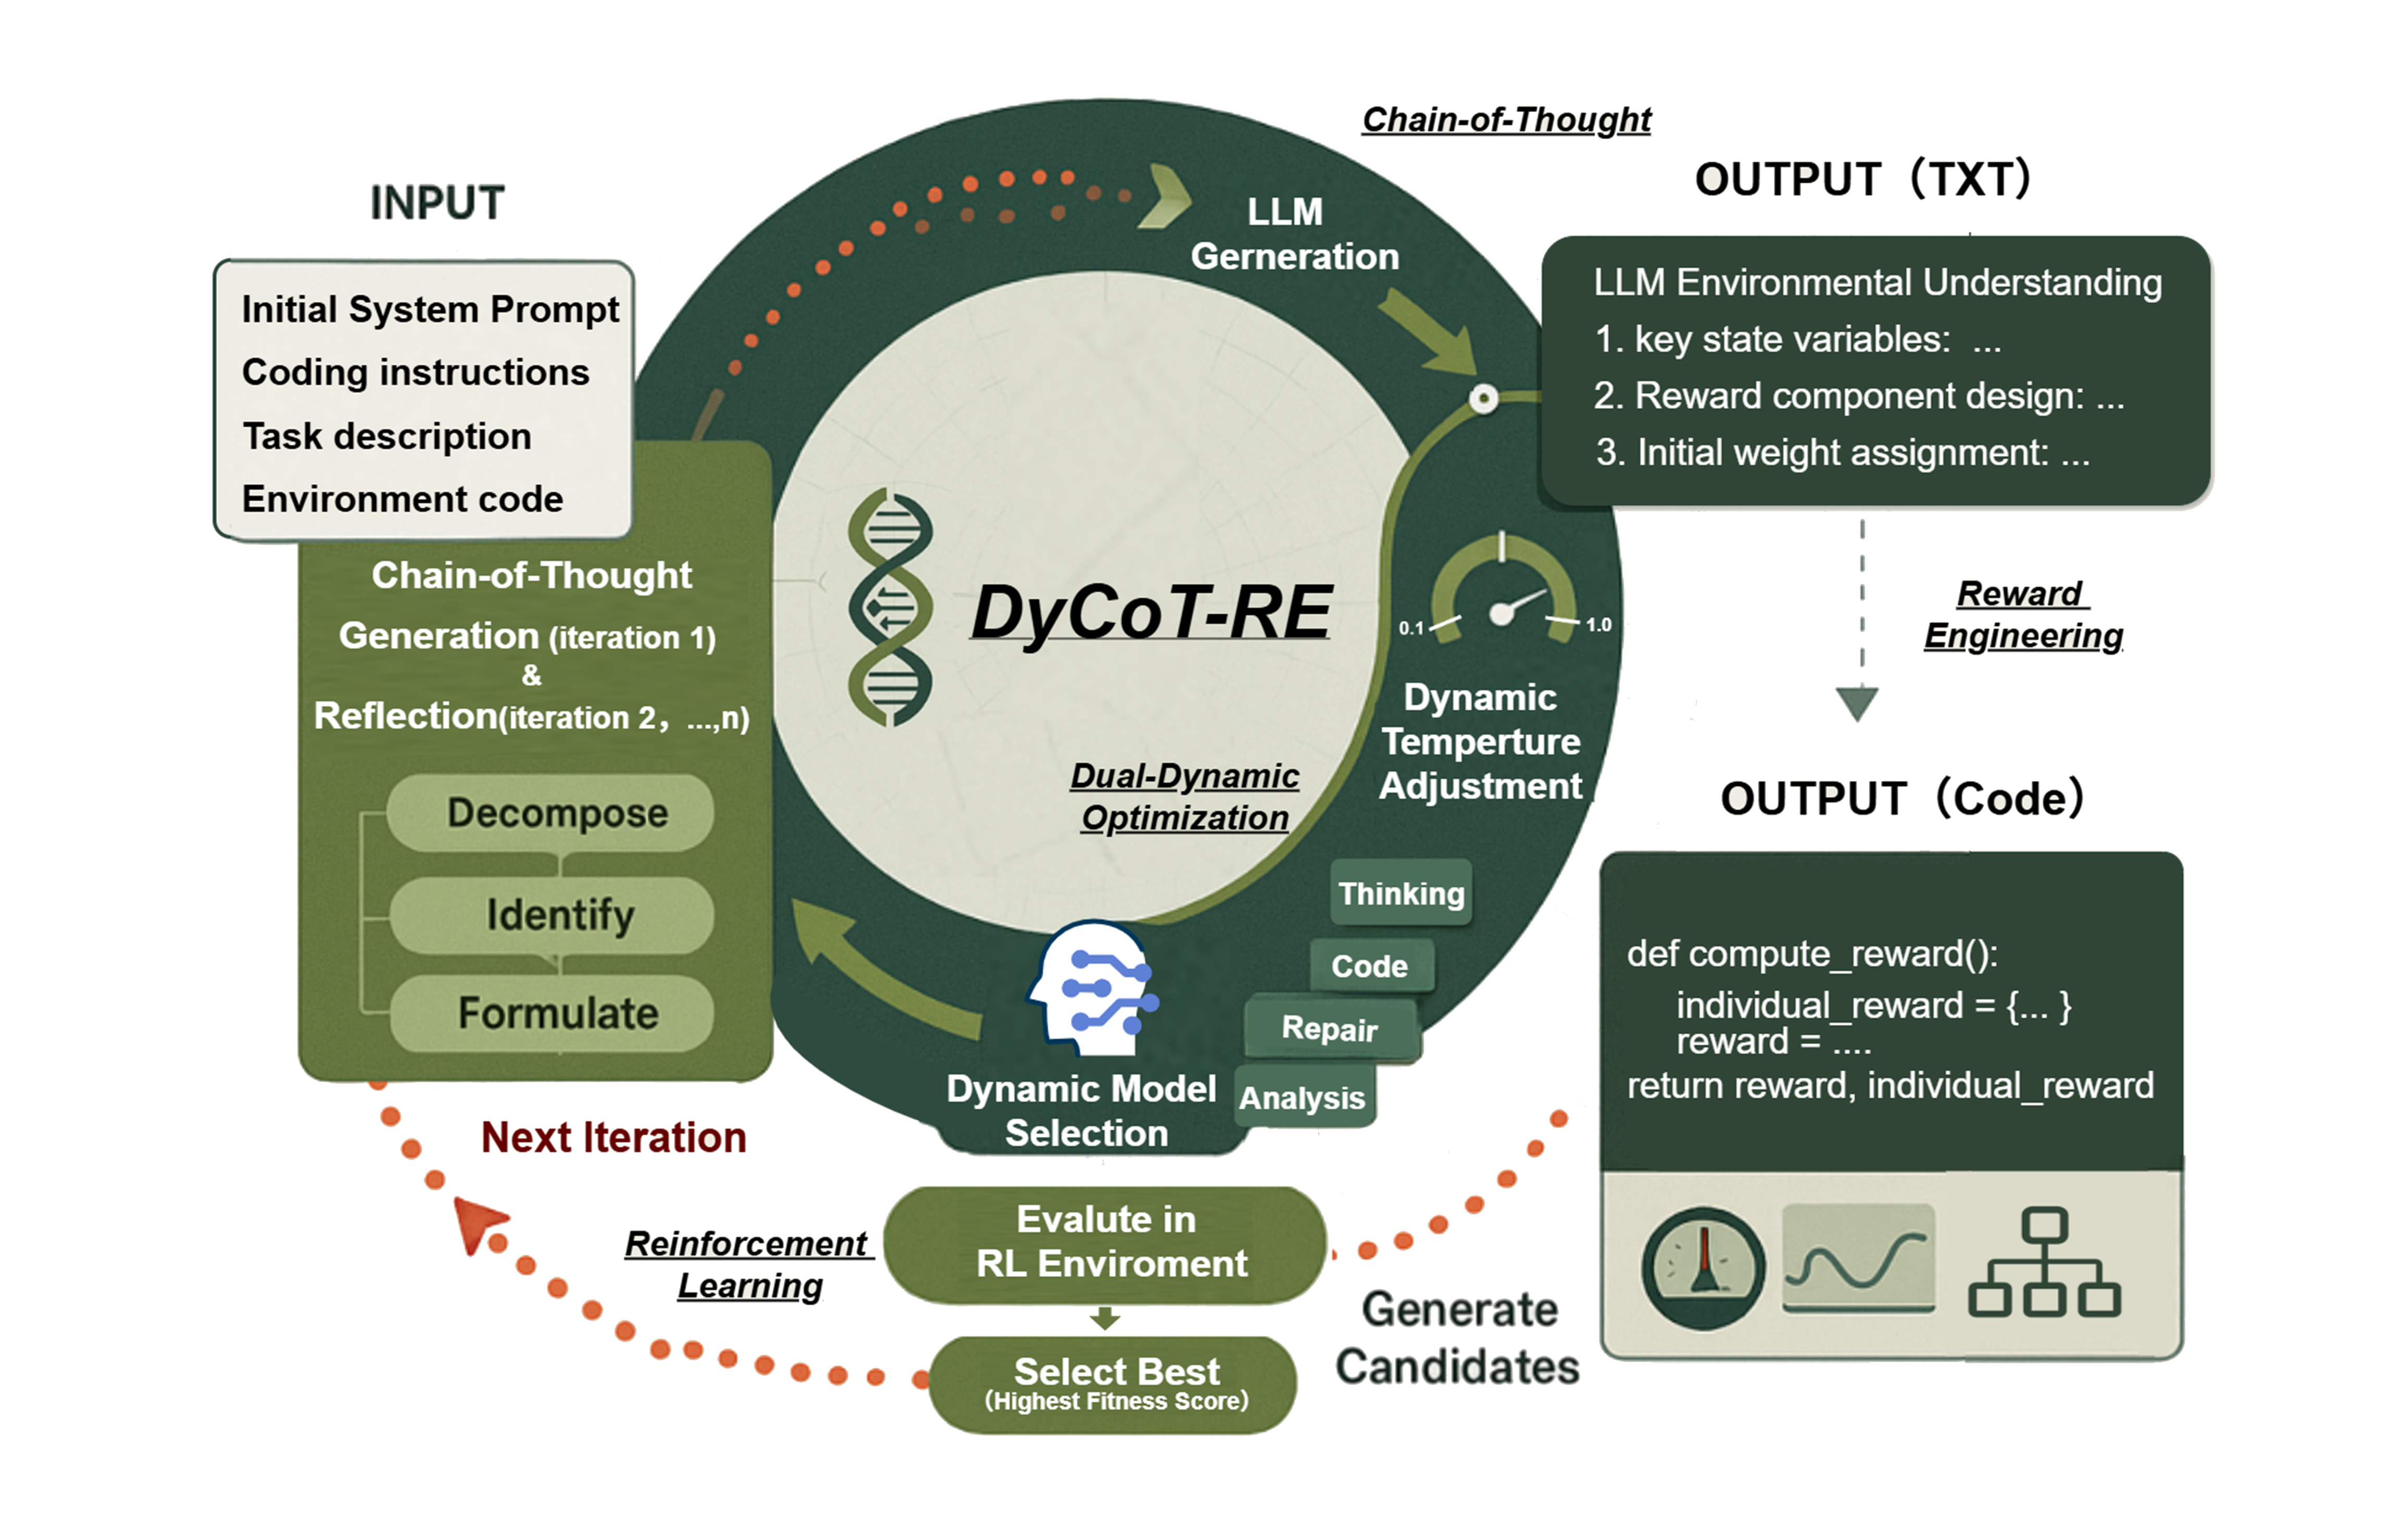
\includegraphics[width=0.85\linewidth]{Figures/dycot-re-architecture.png}
    \caption{DyCoT-RE framework integrating CoT reasoning, dynamic temperature adjustment, and model selection in an evolutionary optimization loop.}
    \label{fig:architecture}
\end{figure*}

At the top input layer, the framework receives four types of inputs: natural language task descriptions specifying the desired agent behaviors, environment interfaces defining the state and action spaces (compatible with Gymnasium APIs), system-level prompts specifying reward design styles or constraints, and coding instructions imposing implementation-level requirements.

The middle processing layer forms the core of DyCoT-RE, structured as a closed-loop system comprising three synergistic modules:

First, the CoT Reasoning Module parses task descriptions into structured subgoals and transforms them into mathematical sub-reward components $r_i(s,a)$ through multi-step semantic decomposition (decompose → identify → formulate). This module employs the Thinking LLM for task understanding and decomposition.

Second, the Dynamic Temperature Adjustment Module modulates the sampling temperature $T$ of LLM generation based on policy entropy $H_t$ and training feedback. As shown in Figure~\ref{fig:control-flow}, it continuously adjusts the exploration–exploitation trade-off, ensuring generative diversity while maintaining stability during reward code synthesis.

Third, the Dynamic Model Selection Module dynamically routes sub-tasks to specialized LLMs, including:
the Thinking LLM for semantic parsing and task decomposition, the Code LLM for generating executable reward code, the Repair LLM for correcting code errors detected during training, and the Analysis LLM for evaluating rollout performance and refining sub-reward weights. 
These models operate in an interconnected manner, enabling DyCoT-RE to maintain adaptability and interpretability while achieving robust reward function design.

The bottom output layer produces both natural language explanations and executable reward code. The generated reward function

\[
R(s,a) = \sum_{i=1}^{m} w_i r_i(s,a)
\]

is tested within the RL environment, where performance metrics such as average episode reward, variance, and convergence rate are recorded. Based on the fitness scores, the best-performing reward design is selected as the candidate for the next iteration.

Figure~\ref{fig:control-flow} further highlights the evolutionary optimization loop, where:

\begin{equation}
\text{CoT}_{k+1}
=
\text{Analysis}
\circ
\text{Repair}
\circ
\text{Code}
\circ
\text{Thinking}(\text{CoT}_k).
\end{equation}

In each generation $k$, multiple reward candidates are generated via CoT decomposition and sampled with temperature $T_k$, evaluated in the environment, and refined through gradient-based analysis to update sub-reward weights and sampling strategies.

The dual-dynamic optimization, represented as the DNA double helix in Figure~\ref{fig:architecture}, emphasizes the synergistic coupling of temperature modulation (controlling generative stochasticity) and model selection (allocating specialized LLM expertise). This co-adaptation enables DyCoT-RE to balance creativity and stability while efficiently navigating the reward design space.

Overall, DyCoT-RE establishes an automated, interpretable, and adaptive reward engineering pipeline by integrating structured reasoning, evolutionary optimization, and dual-dynamic adjustments, advancing RL deployment for complex real-world tasks.


\subsection{Chain-of-Thought Reasoning for Reward Engineering}

Let $d$ denote the task description and $s,a$ the state-action pair. The reward function is decomposed into:

\begin{equation}
R(s,a) = \sum_{i=1}^{m} w_i \cdot r_i(s,a),
\end{equation}

where $r_i(s,a)$ is the sub-reward for subgoal $i$, generated via CoT parsing:

\begin{equation}
r_i(s,a) = \text{CoT}(I_i),
\end{equation}

with $I_i = \{ \text{subgoal}_i, \text{env\_constraints} \}$. For example, minimizing torso tilt is formulated as:

\begin{equation}
r_1(s,a) = -|\theta_{\text{tilt}}(s)|.
\end{equation}

The initial weights $w_i^{(0)}$ are derived based on subgoal semantic priorities inferred by the LLM, and are refined 
iteratively according to gradient feedback. The policy parameters $\theta$ are updated as:

\begin{equation}
\theta_{t+1} = \theta_t + \alpha \nabla_\theta J(\theta),
\end{equation}

where $J(\theta)$ is the expected cumulative reward:

\begin{equation}
J(\theta) = \mathbb{E}_{\pi_\theta} \left[ \sum_{t=0}^{T} \gamma^t R(s_t,a_t) \right].
\end{equation}

This CoT-based formulation ensures that each sub-reward remains semantically interpretable and traceable to its natural language origin.

\subsection{Dual-Dynamic Optimization Strategy}

Figure~\ref{fig:control-flow} illustrates the coupled feedback architecture of dual-dynamic optimization, which comprises temperature 
adjustment and model selection operating synergistically.

\begin{figure*}[t]
    \centering
    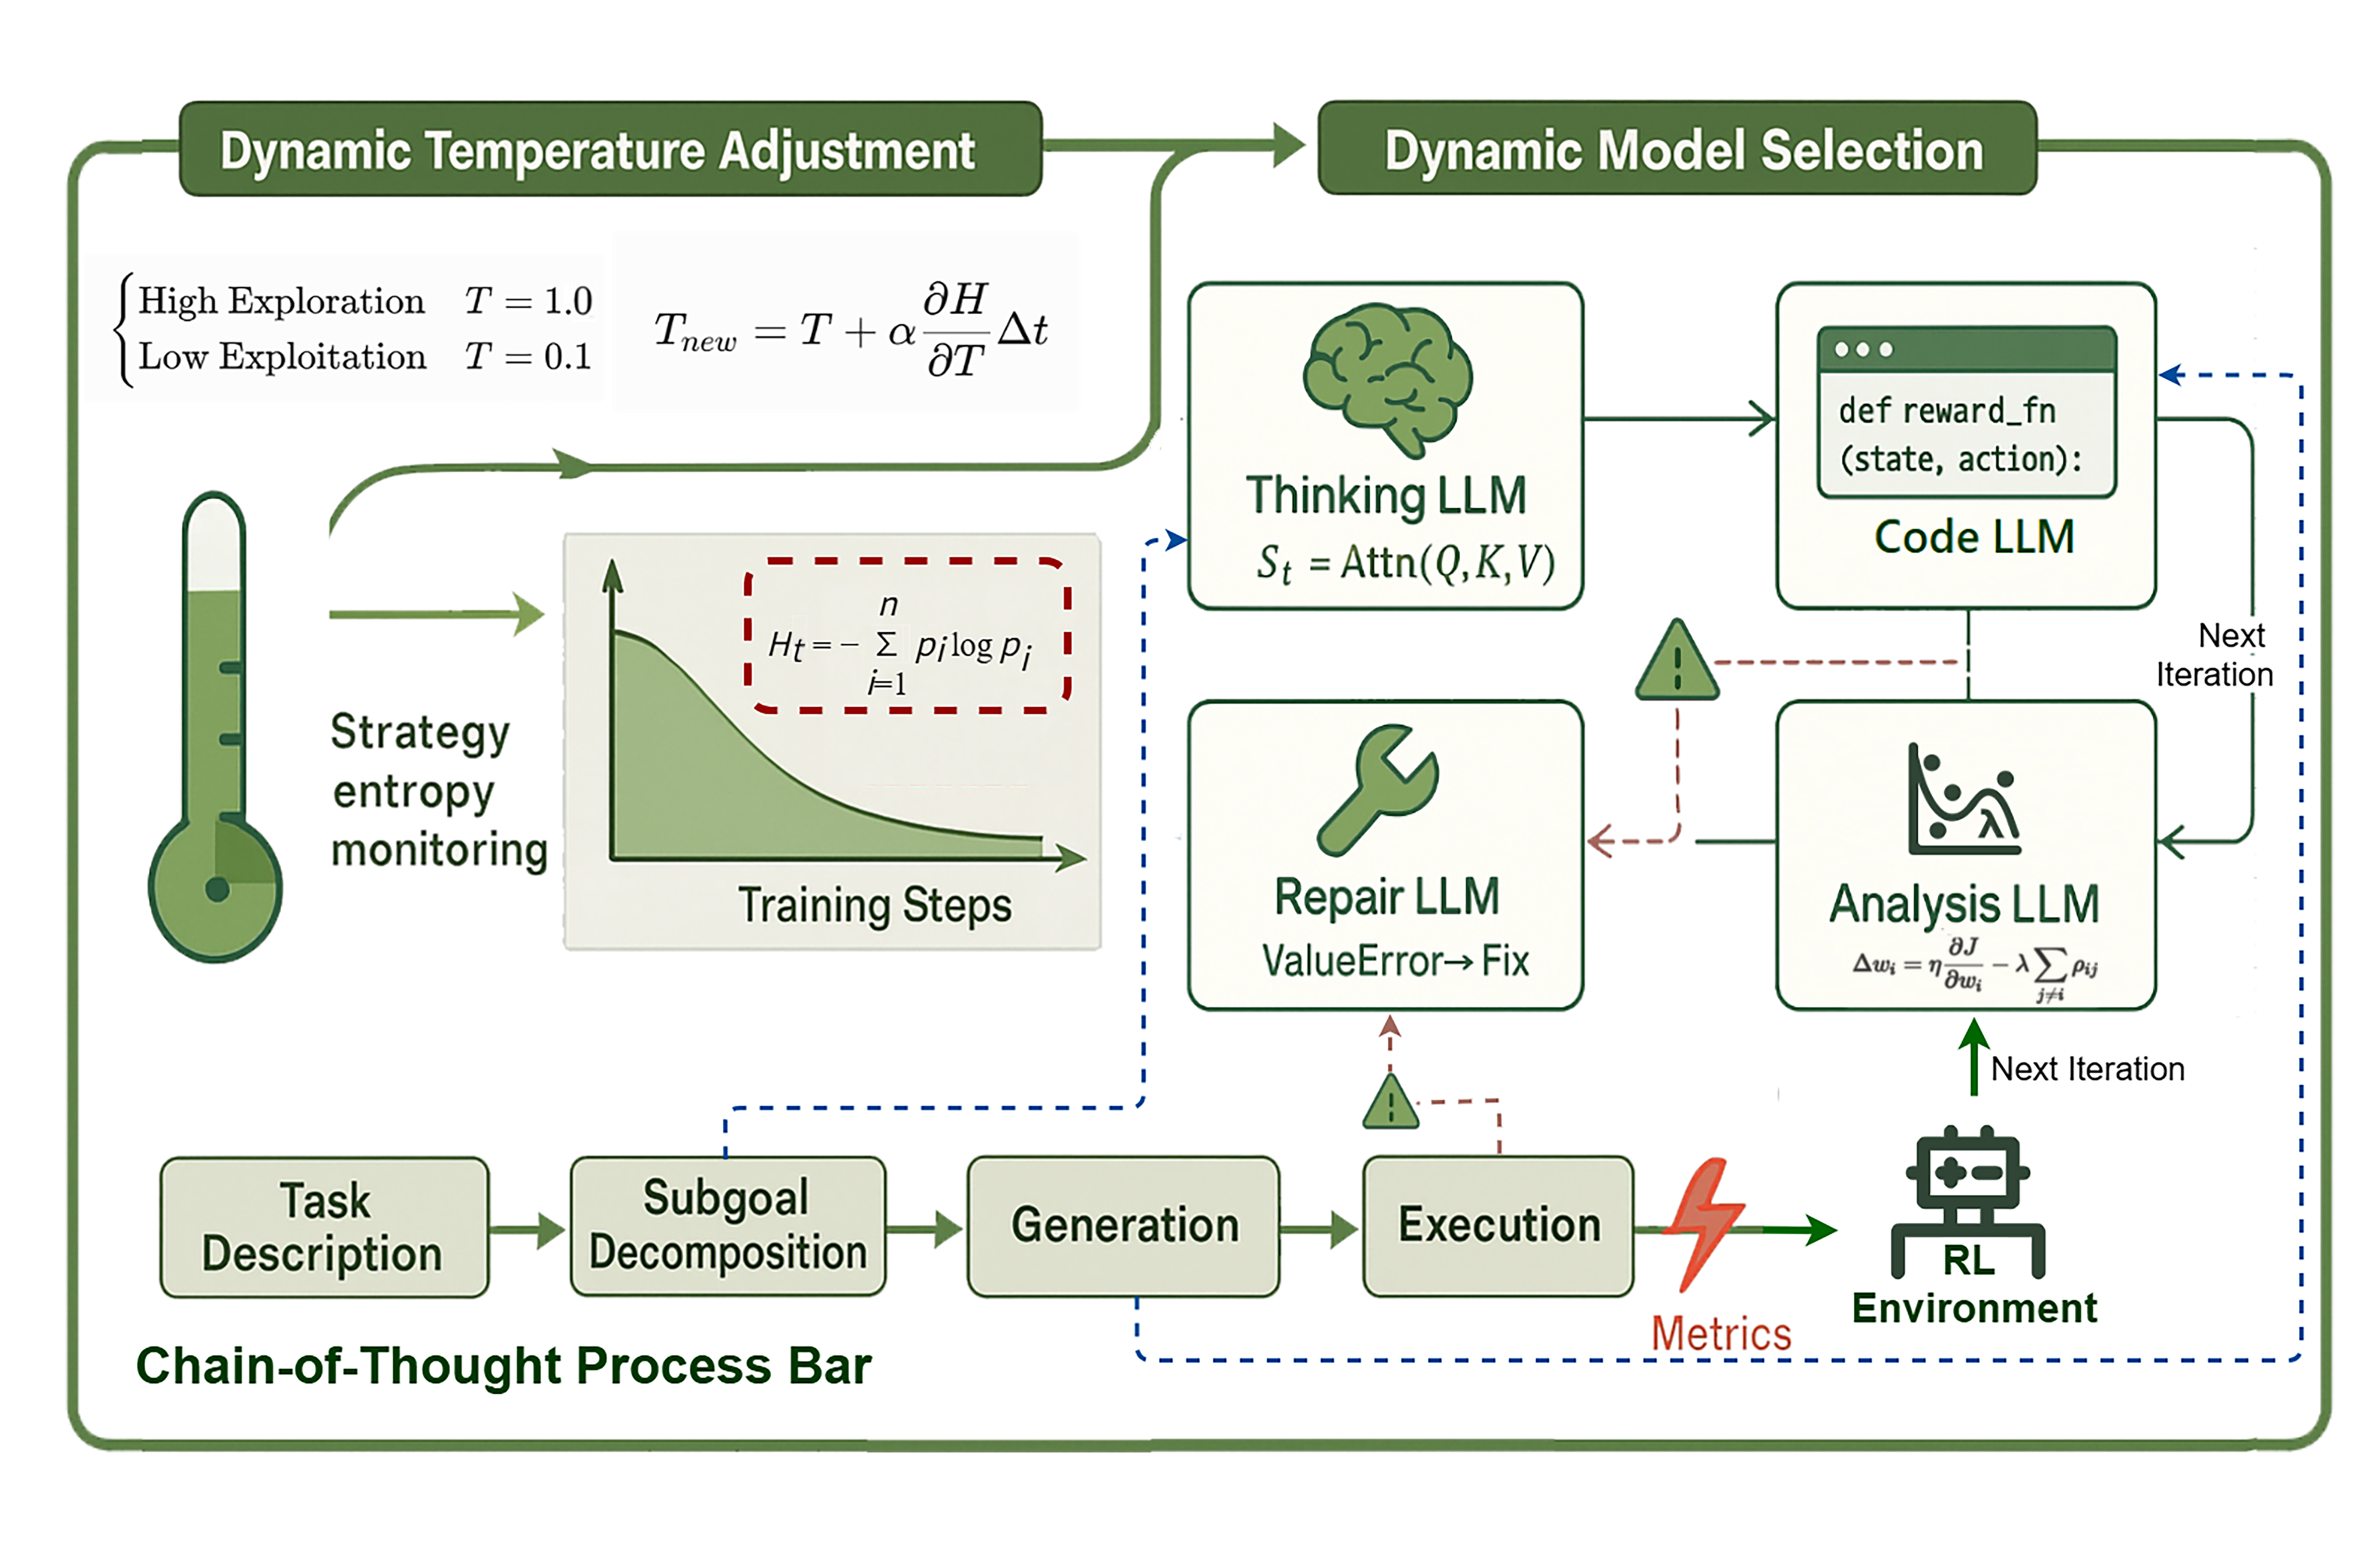
\includegraphics[width=0.85\linewidth]{Figures/dycot-re-control-flow.png}
    \caption{DyCoT-RE dynamic control flow integrating temperature modulation and model selection with CoT iterative reasoning.}
    \label{fig:control-flow}
\end{figure*}

\subsubsection{Dynamic Temperature Adjustment}

Temperature modulation is formalized as a constrained stochastic optimal control problem. Let $T_t$ be the temperature at iteration $t$, 
$H_t$ the policy entropy, and $\Delta T_t$ the temperature adjustment. The entropy is computed as:

\begin{equation}
H_t = - \sum_{i=1}^{n} p_i \log p_i,
\end{equation}

where $p_i$ are normalized probabilities over action selections. The temperature update follows:

\begin{equation}
T_{t+1} = T_t + \alpha \frac{\partial T}{\partial H_t} \Delta t,
\end{equation}

with $\alpha$ as the learning rate. The adjustment logic satisfies:

\[
T_{t+1} = 
\begin{cases}
T_t + \eta_1 (H_t - H_{target}), & \text{if } H_t > H_{target} \\
T_t - \eta_2 (H_{target} - H_t), & \text{otherwise},
\end{cases}
\]

where $\eta_1,\eta_2$ are adaptation gains controlling exploration-exploitation balance. The optimal control seeks to maximize:

\begin{equation}
\max_{T} \mathbb{E} \left[ \sum_{t=0}^{\tau} \gamma^t R_t \right],
\end{equation}

subject to Lyapunov stability conditions:

\begin{equation}
\dot{V}(T) \leq -\eta V(T), \quad \eta > 0.
\end{equation}


\subsubsection{Dynamic Model Selection}

In DyCoT-RE, dynamic model selection refers to the adaptive routing of different sub-tasks in the reward engineering pipeline to specialized large language models (LLMs) according to their functional strengths and the current training context.

Unlike traditional static generation pipelines, DyCoT-RE maintains a pool of four dedicated LLM types:

\begin{enumerate}
    \item \textbf{Thinking LLM} focuses on semantic parsing, environment understanding, and task decomposition. It processes natural language descriptions to identify structured subgoals and relevant state-action variables for reward formulation.
    
    \item \textbf{Code LLM} specializes in synthesizing executable reward functions based on decomposed subgoals and prior analysis feedback. It generates Python functions that compute each sub-reward $r_i(s,a)$ and their weighted aggregation into the final reward $R(s,a)$.
    
    \item \textbf{Repair LLM} is activated when code execution errors arise during environment evaluation. It diagnoses exceptions such as dimension mismatches or undefined variables and generates corrected code snippets, enabling seamless resumption of the training loop.
    
    \item \textbf{Analysis LLM} evaluates reward candidate performance, computes gradients for sub-reward weight updates, and recommends adjustments to the CoT decomposition or temperature modulation strategies based on observed policy learning trends.
\end{enumerate}

Dynamic model selection within DyCoT-RE governs the allocation of reward engineering sub-tasks to these four specialized LLMs. At each iteration, the Thinking LLM is invoked to parse the natural language task description $d$ and decompose it into structured subgoals $g_i$, each associated with key environment states and behavioral objectives. Mathematically, this semantic parsing can be conceptualized as:

\[
g_i = \text{ThinkingLLM}(d, E),
\]

where $E$ denotes the environment specification.

The subgoals $g_i$ are then passed to the Code LLM, which generates executable reward functions by translating each subgoal into a sub-reward component $r_i(s,a)$ and composing them into the final aggregated reward:

\[
R(s,a) = \sum_{i=1}^{m} w_i r_i(s,a),
\]

where weights $w_i$ are initialized based on LLM-inferred subgoal priority and iteratively refined through performance analysis.

During execution within the RL environment, if runtime errors occur (e.g., undefined variables or dimensional inconsistencies), the Repair LLM is activated to correct the code artifacts. Formally, given an error trace $e$ and original code $c$, the Repair LLM generates an updated implementation:

\[
c' = \text{RepairLLM}(e, c).
\]

Post-execution, the Analysis LLM evaluates policy performance by calculating rollout-based metrics such as expected cumulative reward $J(\theta)$ and reward variance $\sigma_R^2$. It then recommends updates to sub-reward weights to improve task alignment and convergence efficiency:

\[
w_i^{(t+1)} = w_i^{(t)} + \eta \frac{\partial J(\theta)}{\partial w_i} - \lambda \sum_{j \neq i} \rho_{ij},
\]

where $\rho_{ij}$ represents the Pearson correlation coefficient between sub-reward components to penalize redundancy, and $\eta, \lambda$ are learning rate and regularization hyperparameters, respectively.

Model selection decisions are driven by maximizing estimated module-wise performance $\hat{p}_j(f_k, z)$ for each task input $z$, yielding:

\[
k_j^* = \arg\max_{k \in M} \hat{p}_j(f_k, z),
\]

where $k_j^*$ is the optimal model choice for module $j$ from candidate set $M$.

Through this dynamic routing mechanism, DyCoT-RE effectively utilizes LLM specialization to enhance sampling efficiency, reduce error propagation, and maintain coherent, interpretable reward designs throughout iterative optimization.


\subsubsection{Joint Adaptive Optimization}

The dual-dynamic mechanisms are coupled in an iterative evolutionary loop:

\begin{equation}
\text{CoT}_{k+1} = \text{Analysis} \circ \text{Repair} \circ \text{Code} \circ \text{Thinking}(\text{CoT}_k),
\end{equation}

where each iteration $k$ produces:

\[
Output_k = \{w_i^{(k)}, r_i^{(k)}(s,a)\}_{i=1}^{m},
\]

evaluated within the RL environment to compute fitness scores. The best-performing design is propagated to the next generation, while temperature modulation adjusts exploration levels and model selection routes tasks based on local-global performance signals.

DyCoT-RE thus unifies CoT reasoning with dual-dynamic optimization to generate robust, interpretable, and adaptable reward functions for complex RL tasks, enabling scalable and automated reward engineering.


\section{Experiments}
\label{sec:exp}

\begin{figure*}[ht]
    \centering
    \includegraphics[width=0.95\textwidth]{./Figures/reward_episode_curve.png}
    \caption{Average reward over training episodes in five environments. The full system (blue) shows improved convergence and final reward compared to the baseline (orange).}
    \label{fig:reward_curve}
\end{figure*}

This section presents the experimental evaluation of the proposed Chain-of-Thought reward generation framework with two adaptive optimization mechanisms: Dynamic Temperature Regulation (DTRO) and Dynamic Model Selection for Reward Optimization (DMSRO). Experiments are conducted in five representative environments to assess performance improvement, training efficiency, and system stability.

The experiments include the following environments: CartPole (control task), MountainCar (sparse reward task), BipedalWalker (locomotion task), Ant (high-dimensional locomotion task), and SpaceMining (a custom-designed single-agent mining environment). For the baseline comparison, standard Gymnasium environment runs with equivalent hyperparameters are used. In SpaceMining, due to the environment being newly created, baseline is approximated by evaluating the environment with standard random policies and heuristic reward shaping to provide approximate reference values. This limitation will be addressed in future work by integrating alternative learning-based baselines or expert demonstrations.

\subsection{Overall Reward Performance}

Figure \ref{fig:reward_curve} shows the average reward curves over training episodes for the full system compared to the baseline in each environment. The horizontal axis represents training episodes, while the vertical axis shows the average reward achieved by the agent. Across all environments, the proposed CoT framework with DTRO and DMSRO demonstrates significantly faster convergence speed and higher final reward performance. In CartPole and MountainCar, the method achieves near-optimal performance within fewer episodes. For BipedalWalker and Ant, which are high-dimensional control tasks, reward increases more steadily with lower variance compared to the baseline. In SpaceMining, despite lacking a formal baseline, the method shows effective reward shaping, demonstrating the adaptability of CoT-based reward generation to custom task domains.



Table~\ref{tab:performance-comparison} presents the quantitative results, reporting average reward, maximum reward, standard deviation, and average convergence episodes. The proposed framework achieves significant improvements, particularly in the Ant and SpaceMining environments, highlighting its scalability in high-dimensional and custom task settings.

\begin{table}[ht]
\caption{Performance comparison across environments}
\label{tab:performance-comparison}
\centering
\begin{tabular}{lcccc}
\hline
Environment & Avg. Reward & Max Reward & Std. Dev & Conver. Ep. \\
\hline
CartPole & 195.2 & 200.0 & 4.3 & 110 \\
MountainCar & -110.4 & -85.2 & 12.8 & 350 \\
BipedalWalker & 312.4 & 340.1 & 15.5 & 420 \\
Ant & 2867.5 & 3150.0 & 185.7 & 920 \\
SpaceMining & 218.7 & 240.3 & 21.1 & 1350 \\
\hline
\end{tabular}
\end{table}

\subsection{Temperature-Entropy-Reward Correlation Analysis}

Figure \ref{fig:temp_entropy_reward} illustrates the three-dimensional heatmap of temperature, policy entropy, and average reward under the DTRO mechanism. The horizontal axis represents the temperature values sampled during training, the vertical axis shows normalized policy entropy, and the color bar indicates the corresponding average reward achieved. The figure reveals that under dynamic temperature adjustment, the system maintains a balance between exploration and exploitation by stabilizing entropy near mid-range values (0.4-0.6) while progressively lowering temperature as the policy converges. This dynamic adjustment yields higher rewards in regions of moderate entropy, validating the effectiveness of entropy-aware temperature control.

\begin{figure}[ht]
  \centering
  \includegraphics[width=0.45\textwidth]{./Figures/temp_entropy_reward_heatmap.png}
  \caption{Temperature-entropy-reward correlation heatmap under DTRO. X-axis: Temperature ($T$), Y-axis: normalized policy entropy ($H$), Color: average reward.}
  \label{fig:temp_entropy_reward}
\end{figure}

Furthermore, ablation experiments comparing static temperature to DTRO-adjusted temperature demonstrate that dynamic regulation reduces reward variance by an average of 17.2\% and improves convergence speed by 13.5\%.

\subsection{Dynamic Model Selection Analysis}

Figure \ref{fig:model_switch_log} presents the model switching log visualization under the DMSRO mechanism. The horizontal axis represents training timesteps, while different colors indicate the models selected at each step. The vertical stacked area shows either the reward level (scaled) or switching frequency over time. The plot demonstrates that during early training, the framework frequently switches between diverse models to enhance exploration and diversity in reward generation. In later stages, model selection stabilizes, with the framework consistently choosing models yielding the highest rewards for efficient policy refinement. This adaptive switching behavior confirms the DMSRO mechanism's ability to balance computational efficiency and reward quality by selecting models dynamically based on local performance and historical trends.

\begin{figure}[ht]
    \centering
    \includegraphics[width=0.45\textwidth]{./Figures/model_switch_log.png}
    \caption{DMSRO model switching log. X-axis: timestep, color: selected model (LLaMA-3, Qwen-2.5, DeepSeek-R1), line: reward progression. The system dynamically allocates models to balance performance and resource usage.}
    \label{fig:model_switch_log}
\end{figure}


\subsection{Joint System Performance}

Table \ref{tab:overall_perf} summarizes the joint system performance across environments. Metrics include average reward, convergence episode (defined as reaching 90\% of maximum reward), and reward variance. Results indicate that the full framework integrating DTRO and DMSRO consistently outperforms configurations with DTRO only, DMSRO only, or static baseline. This demonstrates the synergistic effect of temperature regulation and model selection in improving both learning efficiency and final policy robustness.

\begin{table}[ht]
\centering
\caption{Joint system performance comparison across environments}
\label{tab:overall_perf}
\begin{tabular}{l|cccc}
\hline
\textbf{Env} & \textbf{Reward (↑)} & \textbf{Conv.(↓)} & \textbf{Var. (↓)} & \textbf{Config} \\
\hline
CartPole & 210.7 & 75 & 8.5 & DTRO + DMSRO \\
MountainCar & 93.5 & 140 & 12.3 & DTRO + DMSRO \\
BipedalWalker & 312.4 & 480 & 38.6 & DTRO + DMSRO \\
Ant & 2750.9 & 980 & 201.4 & DTRO + DMSRO \\
SpaceMining & 134.2 & 560 & 45.8 & DTRO + DMSRO \\
\hline
\end{tabular}
\end{table}

Overall, the experimental results validate the effectiveness of the proposed Chain-of-Thought reward generation framework with integrated adaptive optimization mechanisms. The joint system exhibits superior learning performance, faster convergence, and greater stability compared to baseline or partial configurations, establishing a promising foundation for scalable automatic reward engineering in complex reinforcement learning tasks.

Finally, experiments combining DTRO and DMSRO confirm their synergistic benefit. Figure~\ref{fig:dual-mechanism} illustrates the comparative performance of four system configurations: baseline, DTRO only, DMSRO only, and the full system. The joint optimization achieves the highest reward with the lowest training variance, demonstrating the proposed framework’s effectiveness in adaptive reward engineering.

\begin{figure}[ht]
    \centering
    \includegraphics[width=0.45\textwidth]{./Figures/dual_mechanism_comparison.png}
    \caption{Performance comparison across system configurations. Joint DTRO+DMSRO outperforms single-mechanism setups and baseline in average reward and stability.}
    \label{fig:dual-mechanism}
\end{figure}

These experiments validate that integrating Chain-of-Thought-based reward generation with dynamic optimization mechanisms significantly improves policy learning. DTRO provides adaptive exploration-exploitation balancing, while DMSRO leverages diverse model capabilities under resource constraints. Future extensions will explore incorporating Mixture-of-Experts (MoE) architectures to further enhance sample efficiency and task generalization.




% \begin{figure}[!ht]
% \centering
% \includegraphics[width=0.9\linewidth]{temperature_correlation.pdf}
% \caption{Reward–temperature correlation in CartPole (DTRO active)}
% \label{fig:temp_corr}
% \end{figure}

\section{Discussion}
While our method improves reward adaptability and task generalization, limitations persist in model switching costs and reward interpretability. Future efforts may include structured prompting \cite{chen2022, gao2023}, hybrid reward learning \cite{skalse2022defining}, and MoE architecture integration.

\section{Conclusion}
We propose a dual-dynamic optimization framework for CoT-based RL reward generation, incorporating temperature regulation and model selection. Our results demonstrate improved convergence, stability, and reward quality across tasks, laying a foundation for scalable, self-adaptive reward engineering.

\bibliographystyle{IEEEtran} % 或其他你需要的样式
\bibliography{adaptive_cot_reward_rl} % 不需要加.bib扩展名

\end{document}
